\chapter{Planteamiento del problema}

\subsection{Desaparici\'on forzada de personas en México}

\justify
La desaparición forzada de personas en México es una problematica social que se ha encrudeció en años recientes. El Registro Nacional de Datos de Personas Extraviadas o Desaparecidas (RNPED), integra los datos de personas no localizadas en México. Obtenidos a partir de las denuncias presentadas ante la autoridad ministerial correspondiente. Este registro incluye únicamente a las personas que a la fecha de corte, continuan sin ser localizadas.



%\begin{figure}
%  \caption{A picture of a gull.}
%  \centering
%    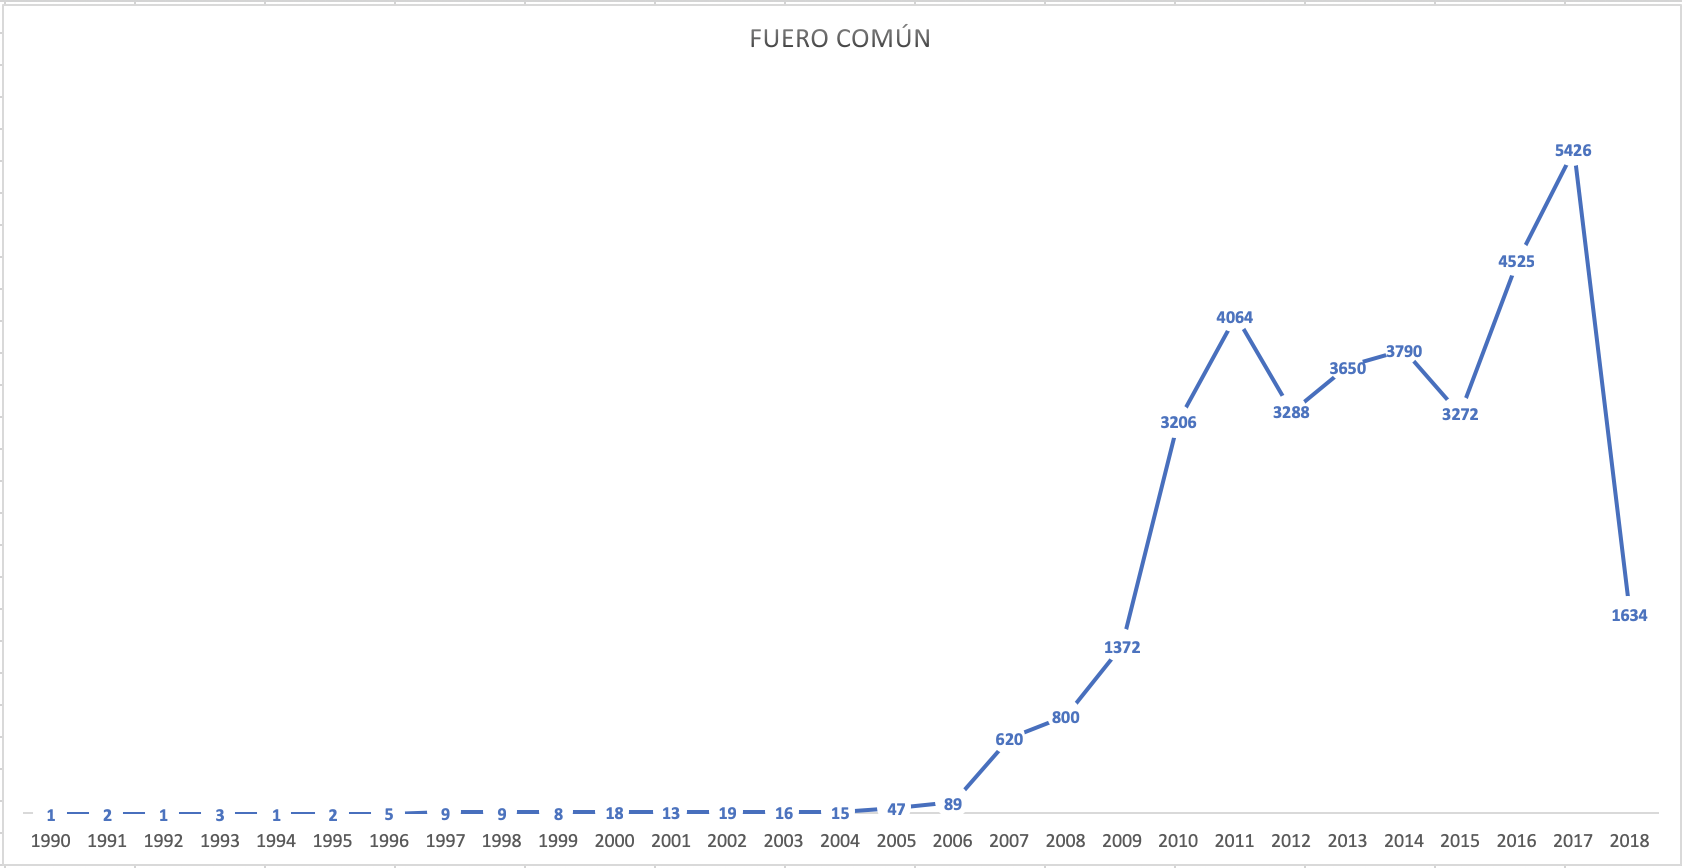
\includegraphics[width=0.5\textwidth]{imgs/fuerocomun}
%\end{figure}

%\begin{figure}
%  \centering 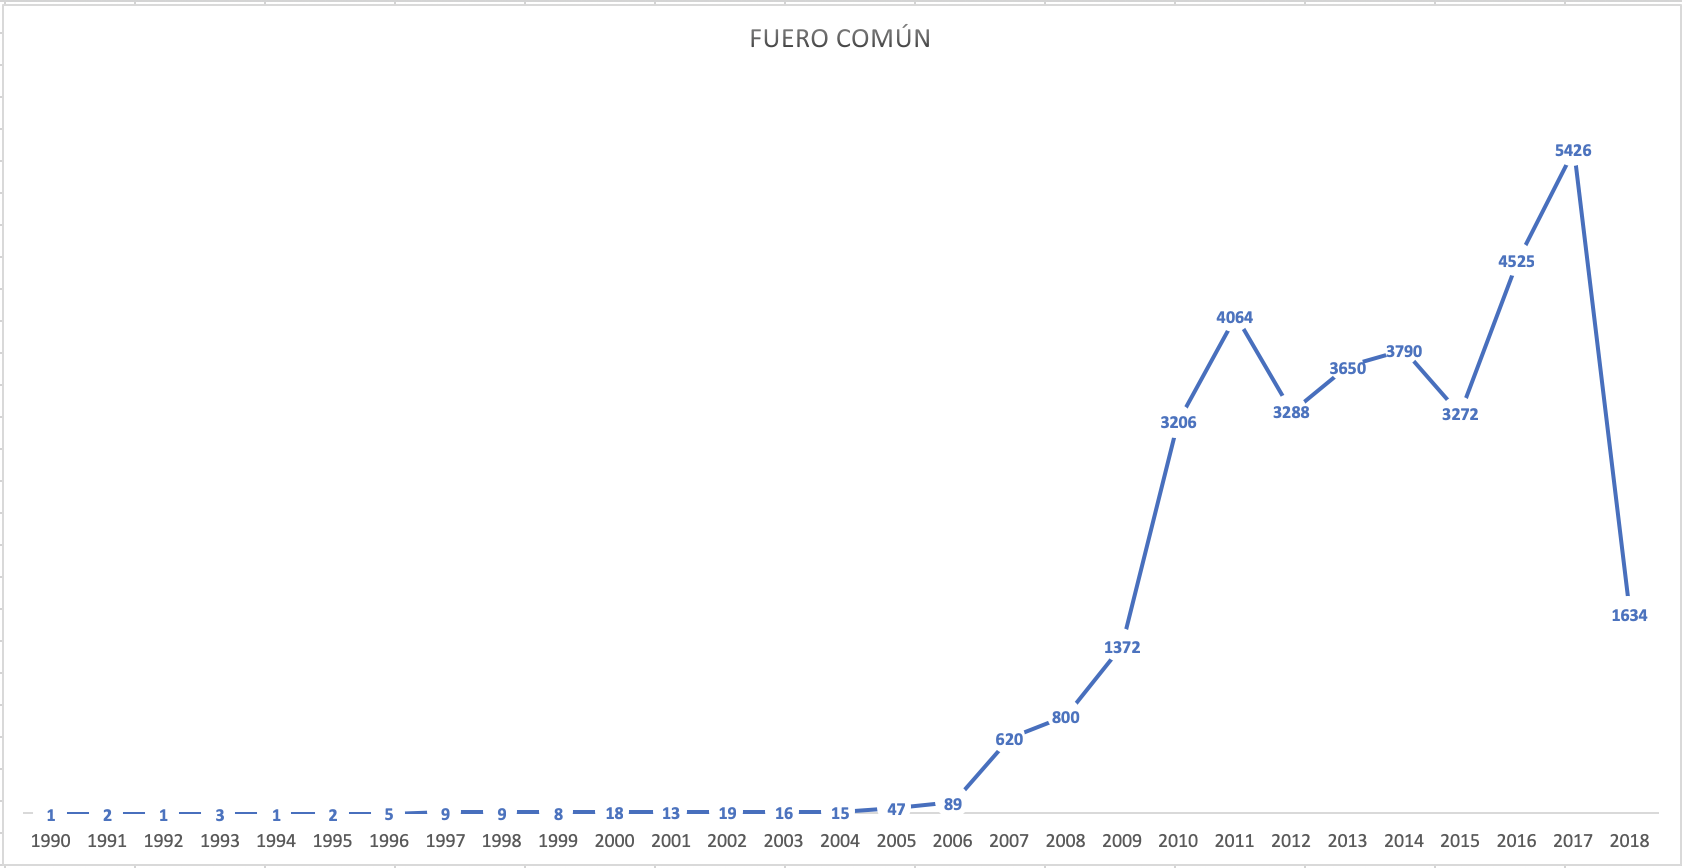
\includegraphics[width=0.3\linewidth]{imgs/fuerocomun.png} \qquad
%  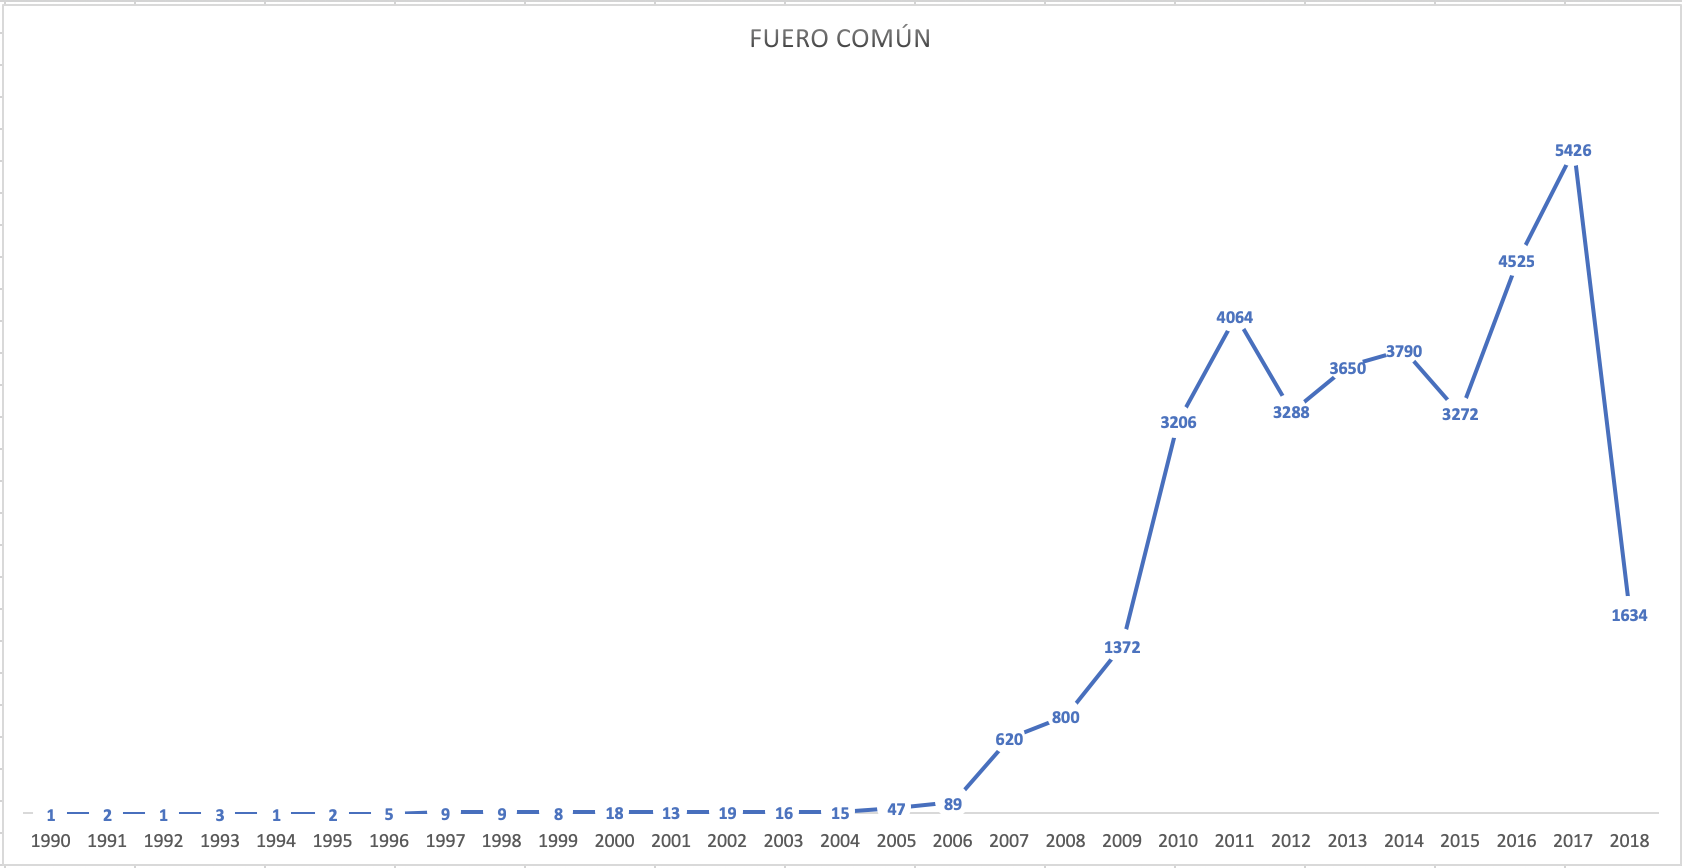
\includegraphics[width=0.3\linewidth]{imgs/fuerocomun.png}
%  \caption{Diagram from Patent Application 12/475,048}
%\end{figure}

\begin{figure}[bp!]
	\centering
	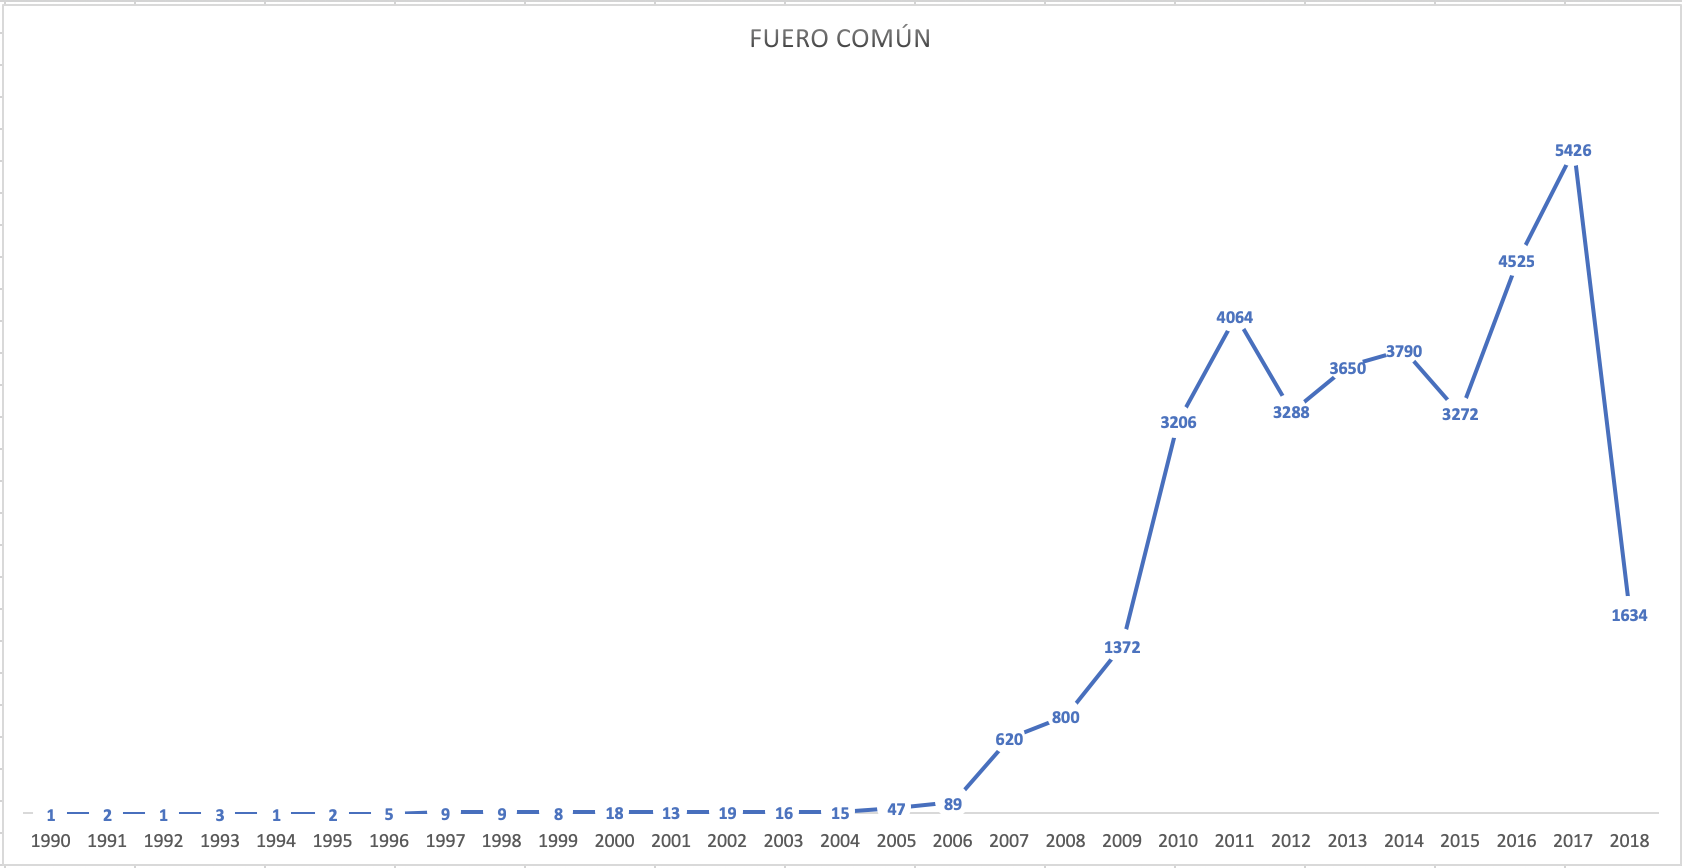
\includegraphics[width=5in]{imgs/fuerocomun}
	  \caption{Estad\'istica Fuero Común}
\end{figure}

\begin{figure}[bp!]
	\centering
	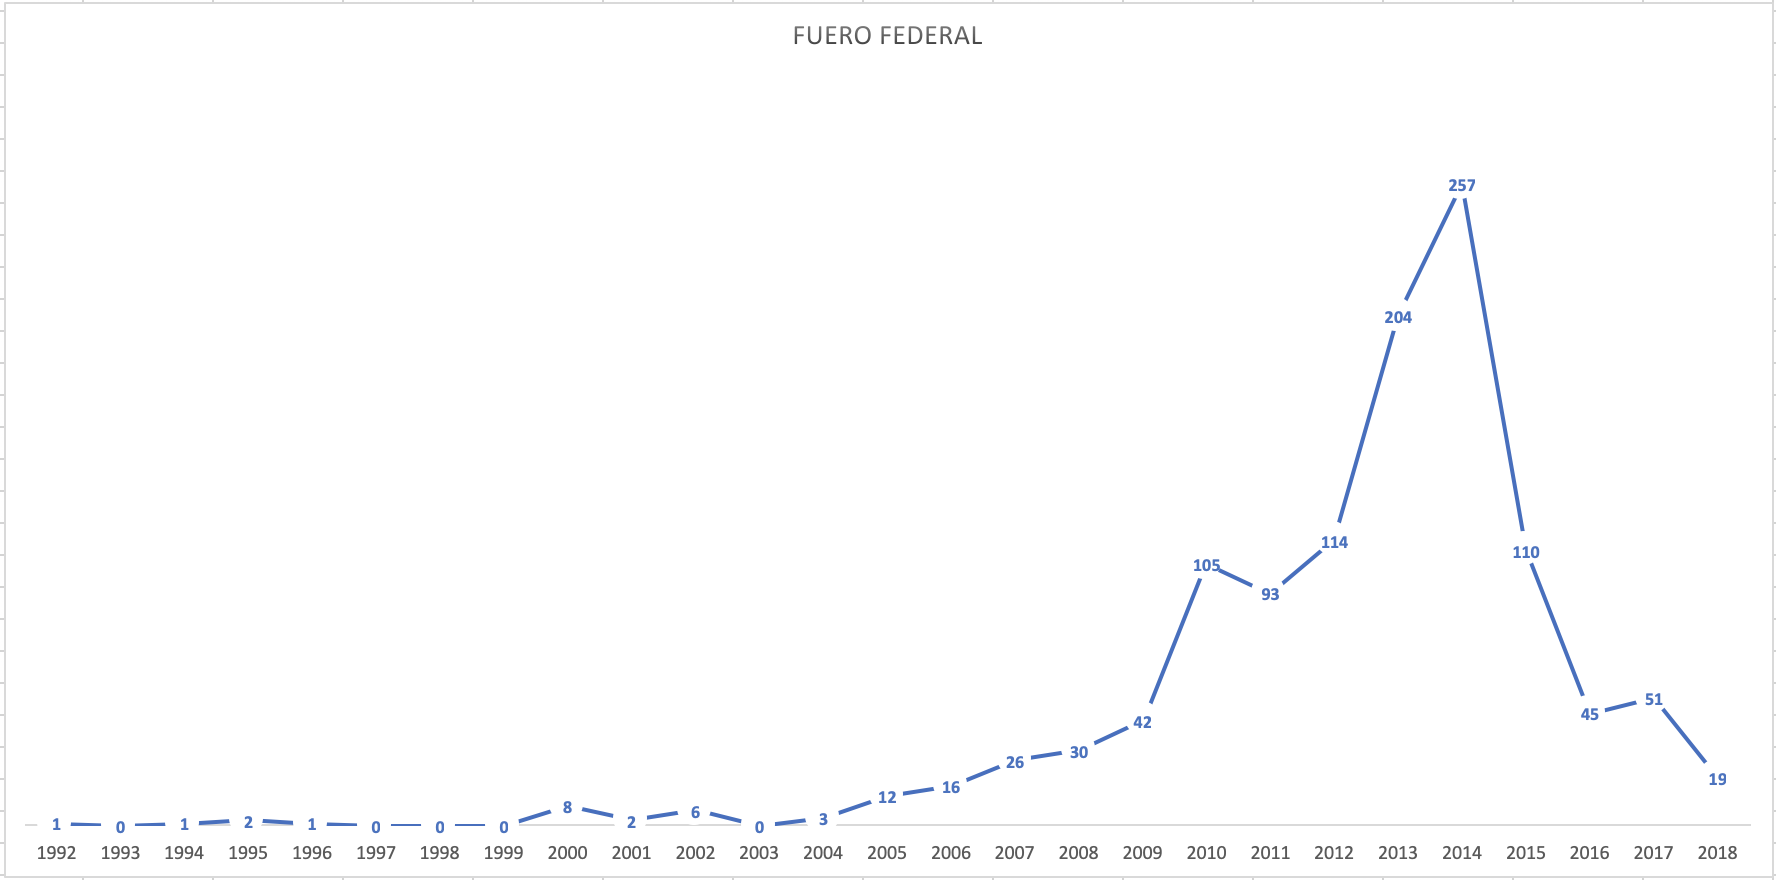
\includegraphics[width=5in]{imgs/fuerofederal}
	  \caption{Estad\'istica Fuero Federal}
\end{figure}


\justify
Se entiende por persona desaparecida a toda aquella que, con base en información fidedigna de familiares, personas cercanas o vinculadas a ella, se le haya dado por desaparecida, en conformidad con el derecho internacional, lo cual puede estar relacionado con: un conflicto armado internacional o no internacional, una situación de violencia o disturbios de carácter interno, una catástrofe natural o cualquier situación que pudiera requerir la intervención de una autoridad pública competente.


\begin{flushleft}
El RNPED se divide en Fuero Com\'un y Fuero Federal.
\end{flushleft}

\paragraph{Fuero Com\'un}
Y cuando se hace referencia al fuero com\'un o local, se hace referencia a la aplicación territorial de las leyes locales, de las entidades federativas. Como el Código Penal del Distrito Federal, Código Civil del Distrito Federal, etc.

\paragraph{Fuero Federal}
En concreto fuero federal se refiere a la correspondencia de aplicación de leyes federales, en un caso concreto a delitos cometidos en territorio que se considera federal o delitos que se encuentran tipificados en los ordenamientos federales como el Código Federal de Procedimientos Penales, como la Ley de Amparo, la Ley Agraria, etc.

%\begin{flushleft}
%Aun que en 2018 se ve disminuido, estos datos se ven influenciados debido a que el RNPED realizo su fecha de corte el 30 de abril por motivos de delegar esta tarea a a la Comisión Nacional de Búsqueda de Personas como lo informan en su página:
%
%Se informa que el Secretariado Ejecutivo del Sistema Nacional de Seguridad Pública realizó por última ocasión la actualización de las bases de datos del Registro Nacional de Datos de Personas Extraviadas o Desaparecidas (RNPD) del fuero común y fuero federal con corte al 30 de abril.
%
%Cabe mencionar que corresponderá a la Comisión Nacional de Búsqueda de Personas la publicación de las subsecuentes bases de datos, de conformidad con la Ley General en materia de Desaparición Forzada de Personas, Desaparición cometida por Particulares y del Sistema Nacional de Búsqueda de Personas, publicado en el Diario Oficial en noviembre de 2017.
%
%Los anteriores datos de personas desaparecidas en México realmente son alarmante por la exploción que se ha dado cómo podemos observar en la gráfica desde 2007.
%\end{flushleft}
En la figura 3.1 y 3.2 se muestran las estad\'isticas de personas desaparecidas por año para el fuero común y el fuero federal correspondientemente. As\'i como en la figura 3.3 vemos la estad\'tica de ambos fueros mezclados.

\begin{figure}[bp!]
	\centering
	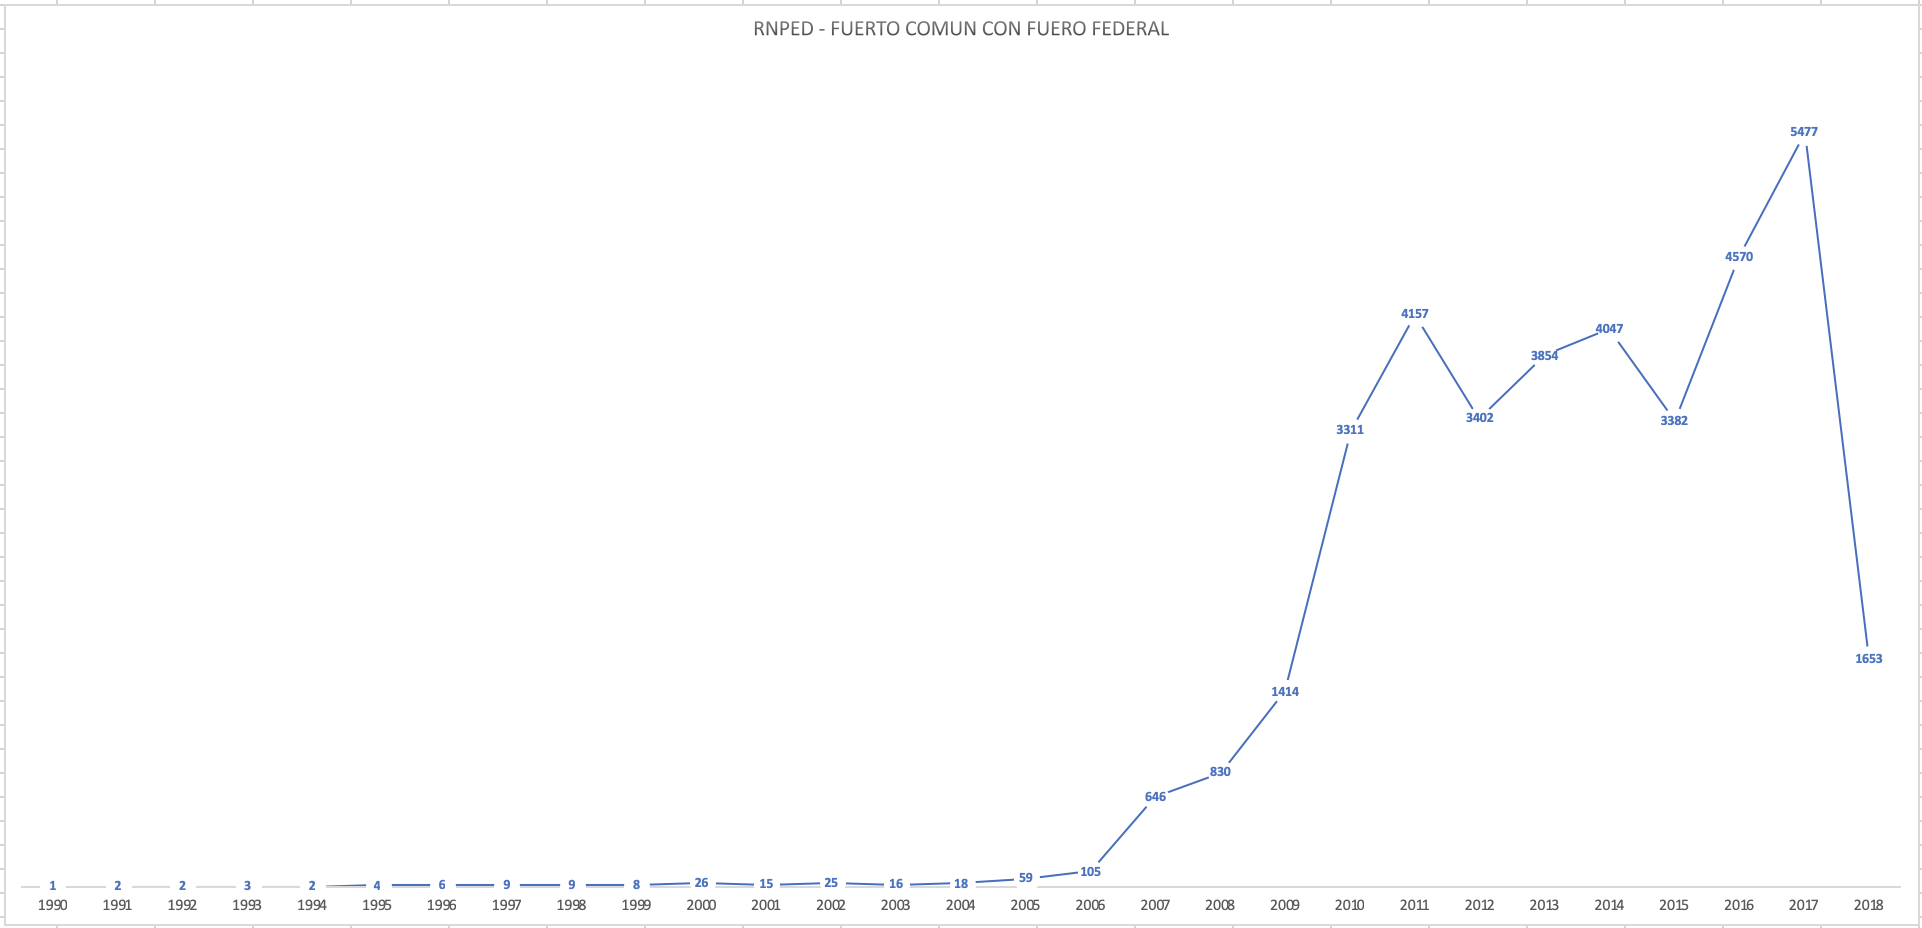
\includegraphics[width=5in]{imgs/fuerocomunYfuerofederal}
	  \caption{Estad\'istica Fuero Común y Fuero Federal}
\end{figure}

En la gr\'afina de la figura 3.3 podemos observar que entre 2006 y 2007 empieza un aumento repentino que alcanza su m\'animo punto en 2017 con 5477 personas desaparecidas. En 2018 se ve disminuido, sin embargo estos datos se ven influenciados debido a que del RNPED realizo su última fecha de corte el 30 de abril de 2018 (en el segundo trimestre del 2018), por motivos de delegar esta tarea a a la Comisión Nacional de Búsqueda de Personas, como lo informan en sus p\'agina:

\begin{quote}
\textit{Se informa que el Secretariado Ejecutivo del Sistema Nacional de Seguridad Pública realizó por última ocasión la actualización de las bases de datos del Registro Nacional de Datos de Personas Extraviadas o Desaparecidas (RNPD) del fuero común y fuero federal con corte al 30 de abril 2018.}
\end{quote}

\begin{quote}
\textit{
Cabe mencionar que corresponderá a la Comisión Nacional de Búsqueda de Personas la publicación de las subsecuentes bases de datos, de conformidad con la Ley General en materia de Desaparición Forzada de Personas, Desaparición cometida por Particulares y del Sistema Nacional de Búsqueda de Personas, publicado en el Diario Oficial en noviembre de 2017.}
\end{quote}


De esta manera no tenemos certeza de del número de desaparecidos en todo 2018 hasta que la Comisi\'on nacional de B\'usqueda de Personas haga p\'publicas sus bases de datos.

Por otra parte Roberto Cabrera Alfaro, Comisionado Nacional de B\'usqueda de Personas, presento su último informe el 17 de enero del 2019. Donde comunica que hasta esa fechas se tiene un registro de 40, 180 personas desaparecidas.

Si sumamos los datos por año desde 2007 seg\'un el RNPED y hacemos la diferencia con el informe de Roberto Cabrera Alfaro, de abril del 2018 a enero del 2019 nos da una cantidad estimada de 4985 desaparecidos en 2018. Lo cual nos habla de que la volumetria de desaparecidos se mantiene.

Para concluir podemos decir que la cifra de desaparecidos en M\'exico en la \'ultima decada (2009-2019) ha incrementado drasticamente y se ha vuelto un problema que necesita ser atendido.

\subsection{Homicidio en México 2018}

Según datos del Instituto Nacional de Estadística y Geografía, INEGI, en la gráfica de la figura 3.4, podemos observar los homicidios ocurridos en territorio nacional desde el año de 1990 a 2017.

Podemos observar que en 2007 llega a su punto más bajo en más de 15 años con 8867 homocidios, apartir de ahí incrementa en más de un 50\% respecto a 2007 llegando a su punto máximo en 2011 con 27213 homicidios (incrementando en más de un 300\% en tan solo 4 años) apartir de ahí baja hasta 2014 con 20010 homicidios, volviendo a subir, para bater record en 2017 con 31174 homicidios, la cifra más alta en más de 25 años, un dato realmente alarmante y que preocupa a la sociedad en general.

Lo anterior afecta directamente a la volumetria de personas desaparecidas, pues posiblemente éstas pertenezca al grupo de personas fallecidas sin identificar. Caso similar si una persona que se encontraba como desaparecida sea allada, pero en calidad de fallecida y disminuya la volumetria y las estadisticas de personas desaparecidas, más sin embargo lo que se busca es la integridad de las personas, es decir, que desaparezcan menos personas y las que se encuentran desaparecidas, se encuentren con vida.

\begin{figure}[bp!]
	\centering
	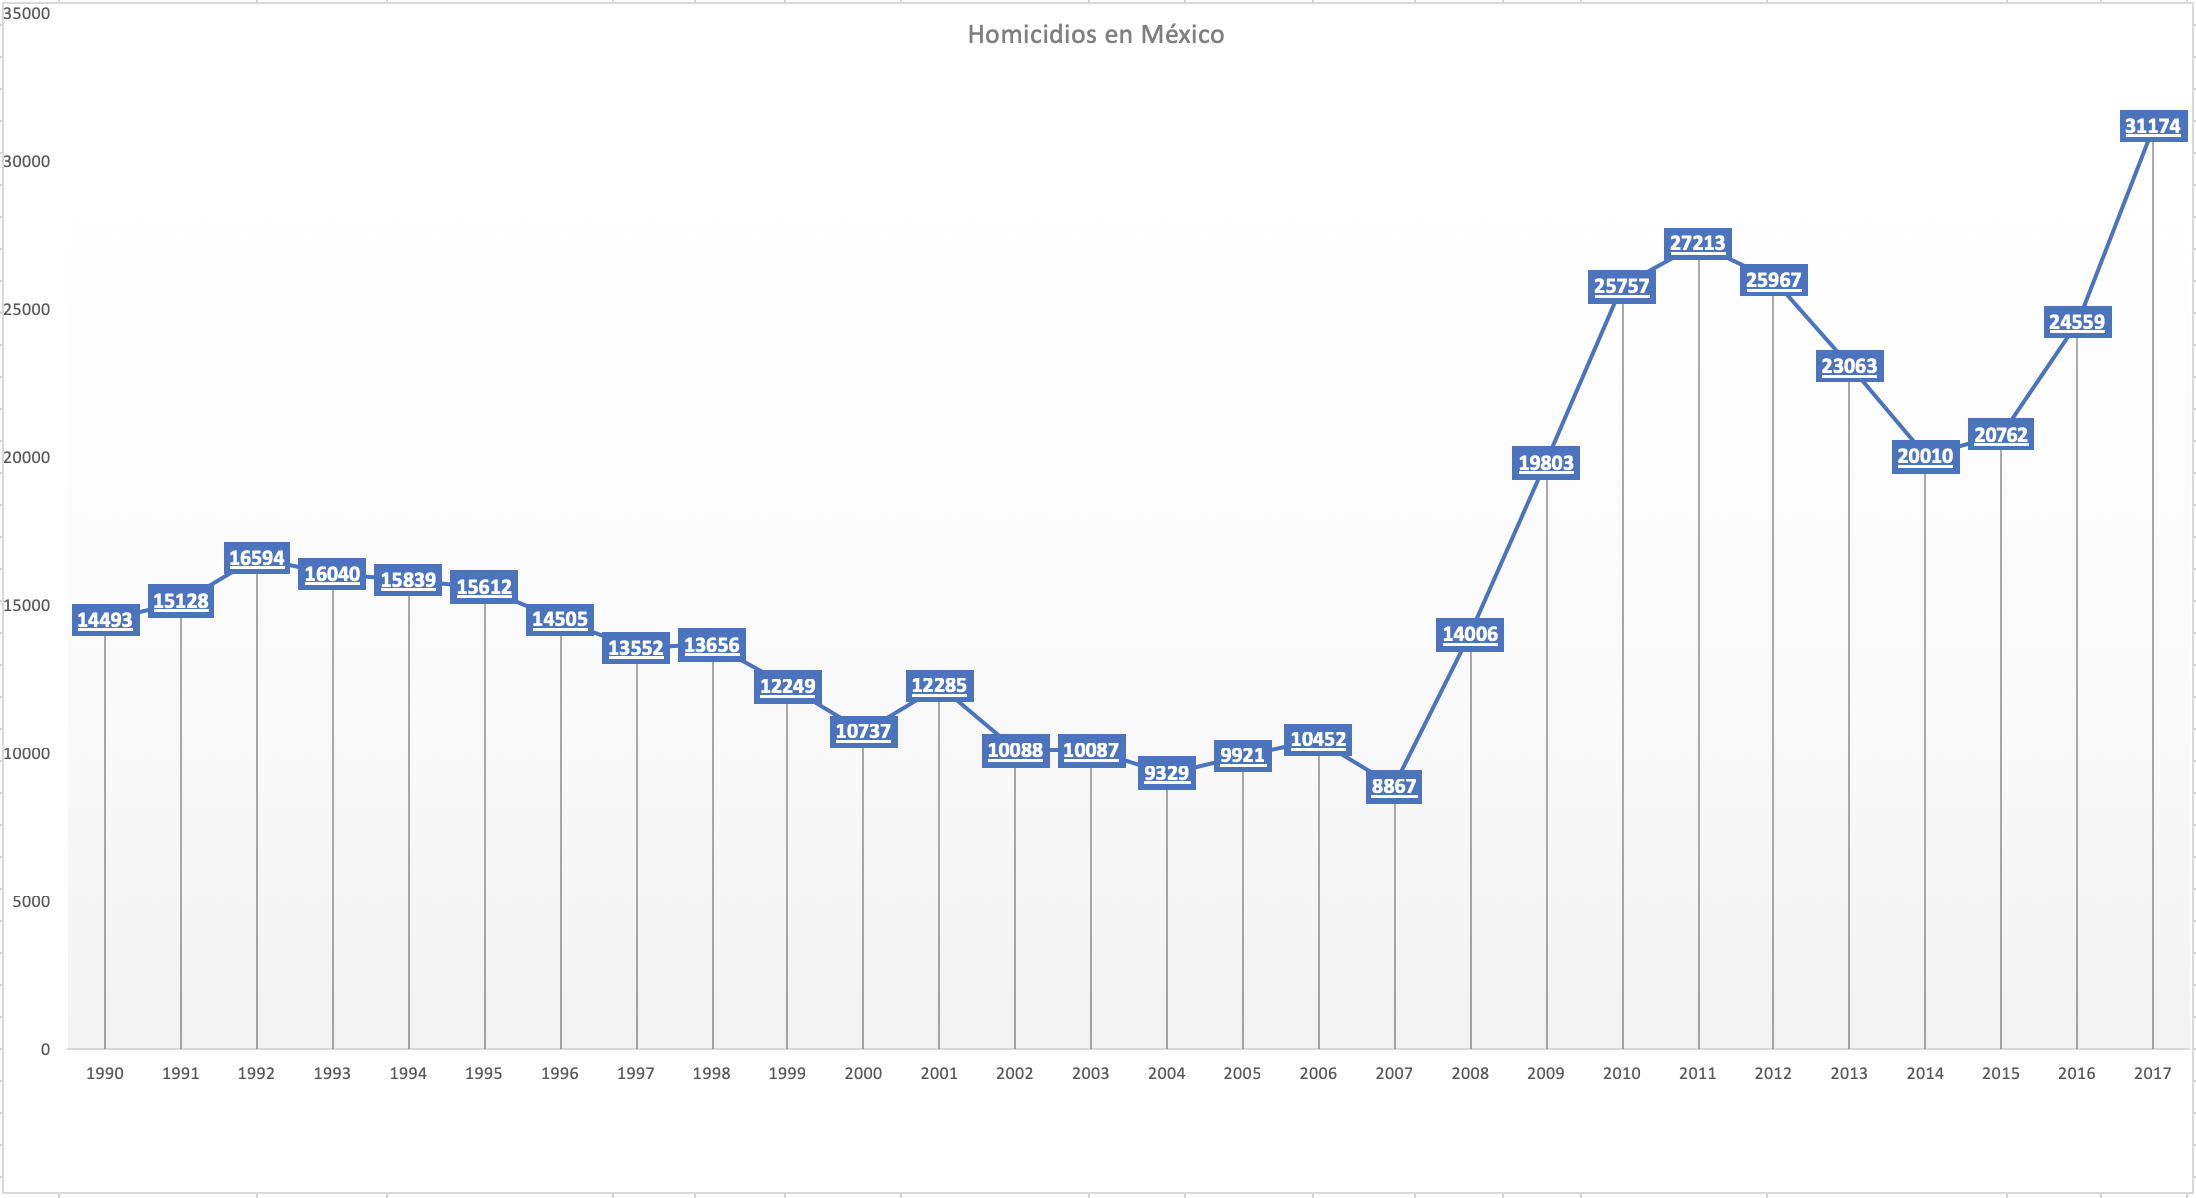
\includegraphics[width=5in]{imgs/homicidios}
	  \caption{Homicidios en México}
\end{figure}

%\newpage
\subsection{Percepción Sobre Seguridad Pública 2018}

Como su nombre lo indica el ENVIPE es la encuesta nacional sobre victimización y persepción sobre seguridad pública. 

Ofrece información referente al nivel de victimización y delincuencia, denuncia del delito, características de las víctimas de delito, los delitos y los daños causados, percepción sobre la inseguridad, desempeño institucional y la caracterización de los delitos en los hogares, entre otros.

Al mismo tiempo se da continuidad a la medición del grado de confianza social en las instituciones de seguridad pública y la percepción sobre su desempeño, los cambios en actividades y hábitos de las personas por temor al delito, la victimización del hogar y la victimización personal, así como a la identificación y medición de las actitudes y experiencias de las víctimas ante las instituciones de seguridad pública y de procuración de justicia.

La ENVIPE mide delitos que afectan de manera directa a las víctimas o a los hogares, tales como: Robo total de vehículo, Robo parcial de vehículo, Robo en casa habitación, Robo o asalto en calle o transporte público, Robo en forma distinta a las anteriores (como Carterismo, Allanamientos, Abigeato y Otros tipos de robo), Fraude, Extorsión, Amenazas verbales, Lesiones y Otros delitos distintos a los anteriores (como Secuestros, Delitos Sexuales y Otros delitos). 

Como podemos observar en 2017 el 29.74\% de la población en México ha sido victima de algún tipo de los delitos de los ya mencionados, redondeando 3 personas de cada 10. Si la taza de violencia sigue aumentando así podriamos decir que promediando las tazas de años anteriores (0.821857143p) para 2021, 1 de cada 3 personas seran victimas de algun tipo de delito de los anteriores mencionados. Lo cual tambien es un dato preocupante.

\begin{figure}[bp!]
	\centering
	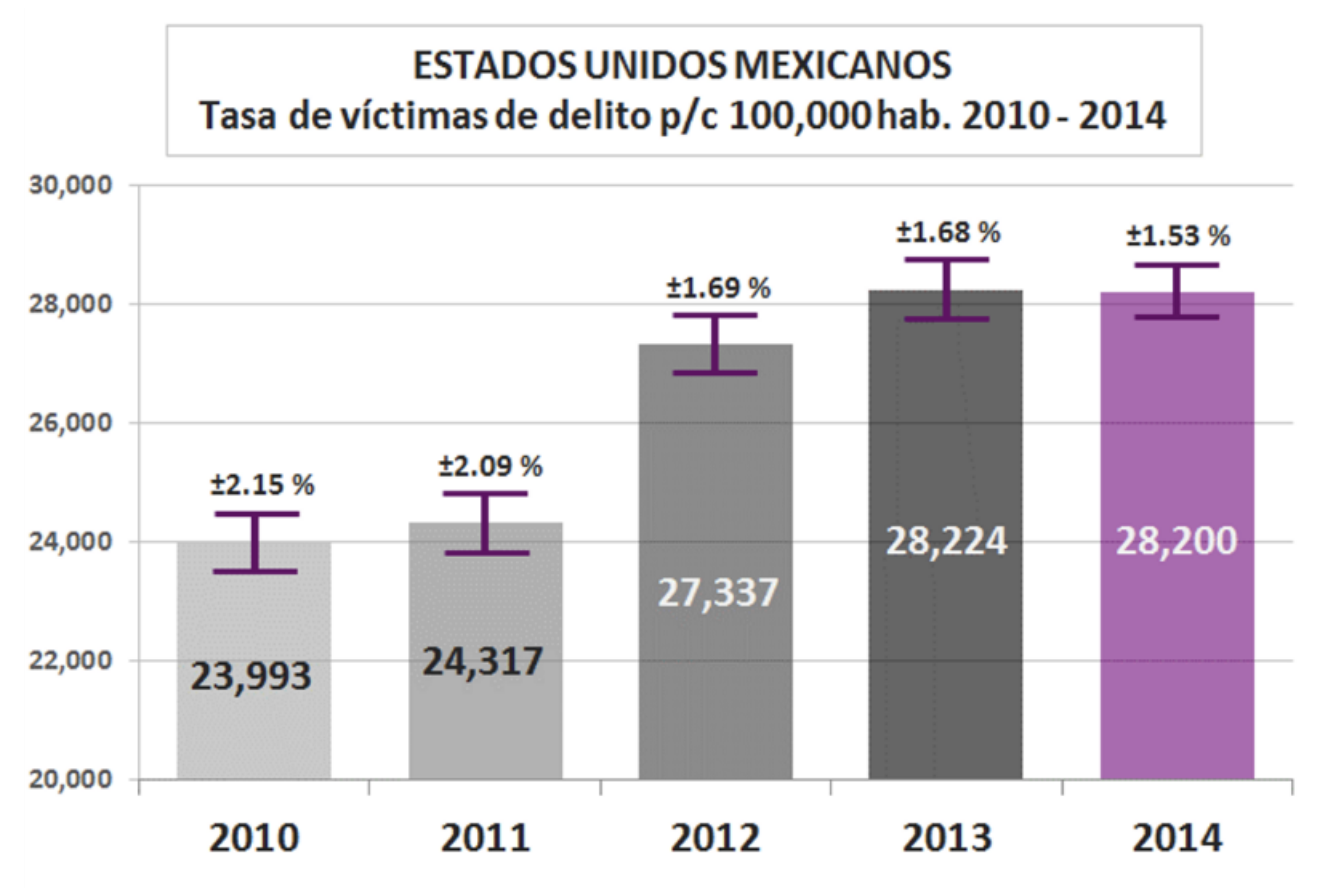
\includegraphics[width=5in]{imgs/envipe2010}
	  \caption{Tasa de v\'intimas de delito p/c 100, 000 habitantes. 2010-2014.}
\end{figure}

\begin{figure}[bp!]
	\centering
	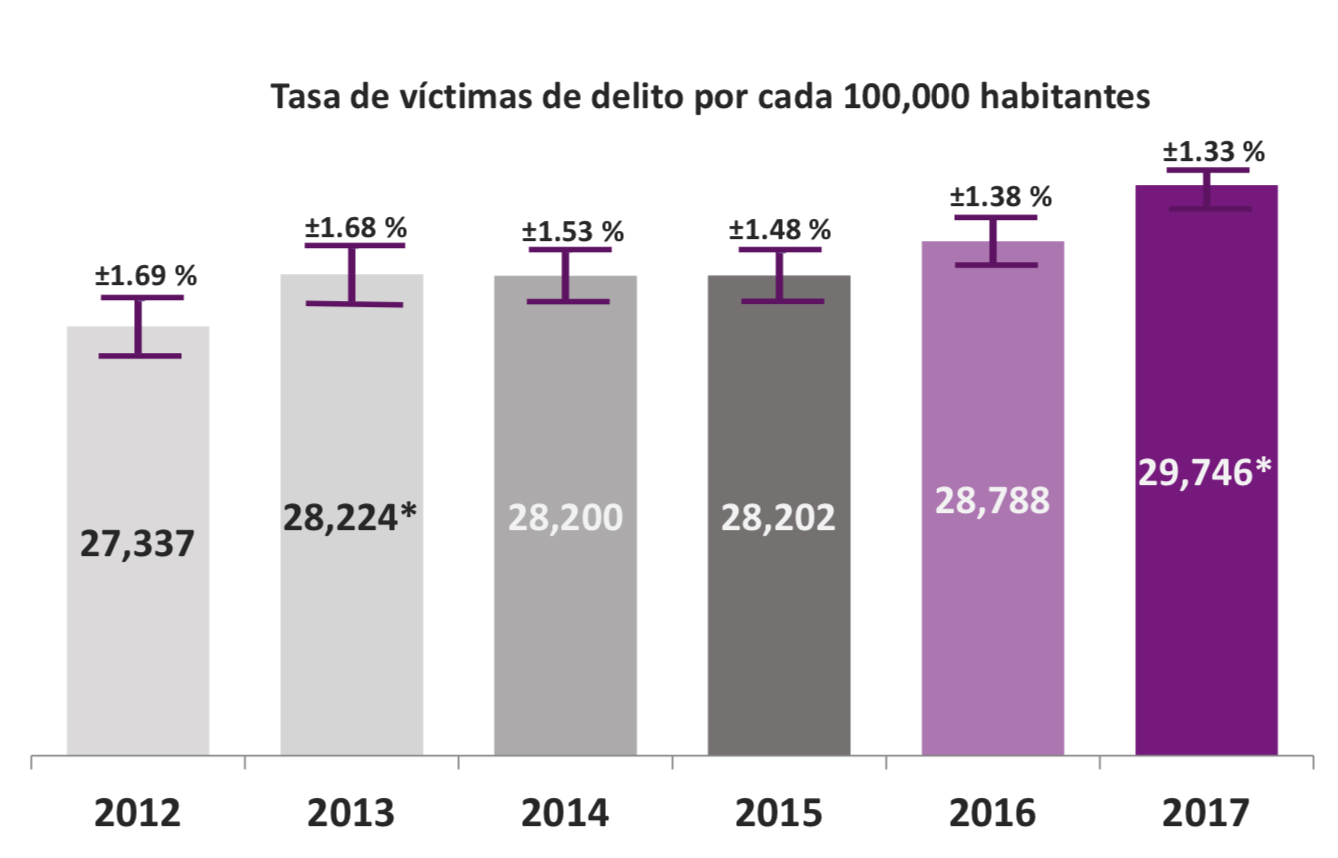
\includegraphics[width=5in]{imgs/envipe}
	  \caption{Tasa de v\'ictimas de delito por cada 100, 000 habitantes. 2012-2017.}
\end{figure}


